\documentclass[10pt, conference, letterpaper]{IEEEtran}

\ifCLASSINFOpdf
	\usepackage[pdftex]{graphicx}
	\graphicspath{{./figures/}}
\else
  \usepackage[dvips]{graphicx}
  \graphicspath{{./figures/}}
\fi
	
\usepackage[cmex10]{amsmath}
\usepackage[caption = false, font = footnotesize]{subfig}
\usepackage{amsthm}
\usepackage{amsfonts}

\newtheorem{theorem}{Theorem}
\newtheorem{lemma}{Lemma}
\newcommand*{\Rom}[1]{\uppercase\expandafter{\romannumeral #1\relax}} % new command to type upper case Roman numbers
%\usepackage[normlem]{ulem}
%\usepackage{algoithm}
%\usepackage{algpseudocode}
\usepackage{textcomp}
\usepackage{gensymb} % include degree mark


\DeclareMathOperator*{\argmax}{arg\,max}
\DeclareMathOperator*{\unif}{unif}
\DeclareMathOperator*{\E}{\mathrm{E}}
\DeclareMathOperator*{\LOS}{\mathrm{LOS}}
\DeclareMathOperator*{\NLOS}{\mathrm{NLOS}}
%\newcommand*\conj[1]{\bar{#1}}
%\newcommand*\mean[1]{\bar{#1}}
\newcommand{\overbar}[1]{\mkern 1.5mu\overline{\mkern-1.5mu#1\mkern-1.5mu}\mkern 1.5mu}


\begin{document}
\title{Indoor mmWave Wearable Networks: Analysis of Large Scale Movements}

\author{\IEEEauthorblockN{Yicong Wang and Gustavo de Veciana}
\IEEEauthorblockA{Department of Electrical and Computer Engineering, The University of Texas at Austin\\Email: yicong.wang@utexas.edu, gustavo@ece.utexas.edu }
}

\maketitle

\section{Related Work}
Channels in dense mmWave wearable networks are sensitive to user movements, including small local movements like turning torso or swinging and large scale movements, e.g., people walking around. Existing work on the user mobility includes \cite{humanactivity}\cite{timevaryingpathshadowing}\cite{blockagein60ghz}, which study the influence of human mobility on the radio channel between fixed transmitter and receiver. 
The authors of \cite{humanactivity}\cite{timevaryingpathshadowing} present measurements of the impact of human mobility on channel variations. 
The work in \cite{timevaryingpathshadowing} further computes the probability that a channel is blocked by users and model the state of channel using a two-state Markov model. 
Authors of \cite{blockagein60ghz} use simulations to get the radio propagation characteristics in the presence of static and moving obstacles and show that directional LOS wave links experience relatively high outage. 
These works provide valuable measurements and insights on the influence of moving human blockage, but lack tractable analysis of user movements to quantify the temporal variation of fixed channels in different scenarios.

\section{Influence of Mobile Blockers on Static Wearable Networks}\label{section:largemobility}
The scenario we consider is the dense user environment, e.g., in a train cart or an airport, where some users are sitting in their seats while other users are moving around them. 

Before describing the system model, we first introduce the following operations on subsets $A, B\in \mathbb{R}^2$ in \cite{stochasticgeometry}, 
\begin{equation*}
\begin{split}
A \oplus B & = \{x+y:x\in A, y\in B\},\\
x + B & = \{x+y:y\in B\}, \mathrm{~for~} x\in \mathbb{R}^2, \\
\check{B} & = \{x: -x \in B\}.
\end{split}
\end{equation*}


Now we present our model for moving blockages. 
We focus on whether the channel between two fixed point is line-of-sight (LOS) channel. 
The fixed devices are at the same height and the blockages are all tall enough to block the channel, thus we assume all users are placed on a 2-D plane. 
There are two fixed users in the network, with their devices located at $0$ and $x$ respectively.
All other users make constant velocity movements towards some fixed orientations and we denote such a model as Constant Velocity Model (CVM).

At time $0$, the locations of users, $\Phi^0 = \{x_i^0\}_i$, follows a homogeneous Poisson Point Process (HPPP) with density $\lambda$, and the orientations of users is independently and uniformly distributed in $[0, 2\pi]$, $\theta_i \sim \unif(0, 2\pi)$. 
Users moves in a fixed orientation at constant velocities $\{s_i\}_i$ and $s_i$'s are independently and identically distributed (i.i.d.).

Assume $A_0^{\theta_i}$ is convex with bilateral symmetric with respect to $u_i$'s orientation $\theta_i$ and the width of $A_0$ is $D_0$. $x_i^t$ is the location of $u_i$ at time $t$, then the area $u_i$ blocks at time $t$, $\Xi_{i}^t$, is given by 
\begin{equation*}
\Xi_{i}^t = x_i^t + A_0^{\theta_i}.
\end{equation*}
From $t$ to $t+\Delta t$, $u_i$ moves from $x_i^t$ to $x_i^{t+\Delta t} = x_i^t + \vec{s}_i\cdot \Delta t$ and we denote the $l_{x_i^t, x_i ^{t+\Delta t}}$ as the trace of the center of $u_i$. The area that $u_i$ covers during $[t, t+\Delta t]$, $\Xi_i^{[t, t+\Delta t]}$, is as follows, 
\begin{equation*} %\label{eq:cover_area}
\Xi_i^{[t, t+\Delta t]} = A_0^{\theta_i} \oplus l_{x_i^t, x_i ^{t+\Delta t} }.
\end{equation*}
Fig. \ref{fig:boolean} illustrates the CVM for mobile blockages.

\begin{figure}
	\centering
	\mbox{\subfloat[]{\label{subfig:trace} 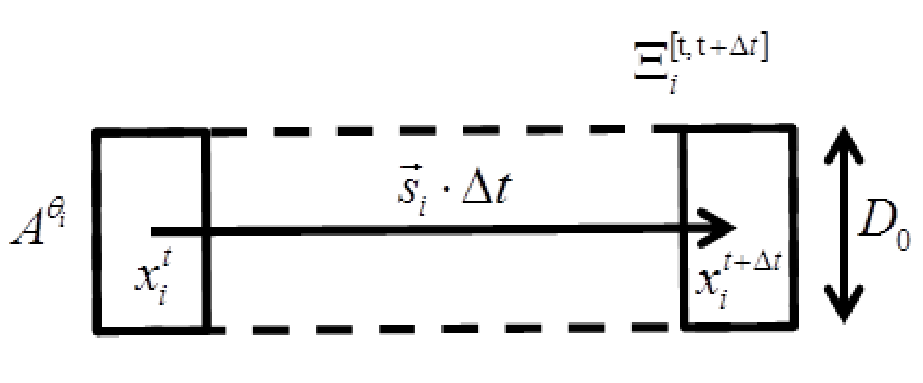
\includegraphics[width=0.3\textwidth]{Channel_trace.pdf}}}
	\mbox{\subfloat[]{\label{subfig:boolean} 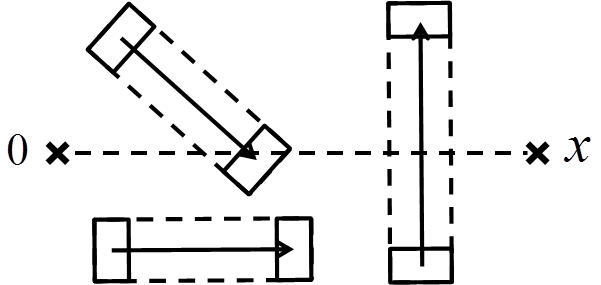
\includegraphics[width=0.3\textwidth]{Channel_boolean.pdf}}}
	\caption[]{\subref{subfig:trace} shows the $\Xi_i^{[t, t+\Delta t]}$, the area $u_i$ covers during $[t, t+\Delta t]$. If $A_0^{\theta_i}$ is convex then $\Xi_i^{[t, t+\Delta t]}$ is also convex. \subref{subfig:boolean} illustrates the area that moving blockages cover during $[t, t+\Delta t]$. $u_i$ has blocked channel in $[t, t+ \Delta t]$ if $\Xi_i^{[t, \Delta t]}\cap x \neq \emptyset$. }
	\label{fig:boolean}
\end{figure}

The distribution of user locations and velocities is given in the following theorem.
\begin{theorem}\label{theorem:boolean_stationary}
Suppose users make i.i.d. constant velocity movements and the locations of users follows HPPP at time $0$, then $\tilde{\Phi}_c^t = \{(x_i^t, (\theta_i, s_i))\}_i$ is stationary.
\end{theorem}
%The proof uses Displacement Theory and is similar to the proof of Theorem \ref{theorem:hppp} and \ref{theorem:hppp_orientation}.
The proof uses the Displacement Theory in \cite{poisson}.

By Theorem \ref{theorem:boolean_stationary}, 
$\Xi_i^{[t, t+\Delta t]}$ is i.i.d. distributed and independent of $x_i^t$ thus we can use the Boolean Model \cite{stochasticgeometry} to model the area that users have covered during $[t, t+\Delta t]$, i.e., 
\begin{equation*}
\tilde{\Phi}_{\Xi}^{[t, t+\Delta t]} = \{(x_i^t, \Xi_i^{[t, t+\Delta t]})\}_i.
\end{equation*}
The set of users that has blocked channel $x$ during $[t, t+\Delta t]$ is given by
\begin{equation*}
N_{\mathrm{B}}^{[t, t + \Delta t]} = \{x_i:x_i \in \Phi, \Xi_i^{[t, t+\Delta t]}\cap x \neq \emptyset \}.
\end{equation*}
For the boolean model, $|N_{\mathrm{B}}^{[t, t + \Delta t]}|$ is a Poisson random variable with parameter $\lambda\mathrm{E}[\nu_2(\check{x}\oplus \Xi_i^{[t, t+\Delta t]})]$, where $\nu_2$ is the area of the set \cite{stochasticgeometry}.

$A_0^{\theta_i}$ is bilateral symmetric, $\theta_i\sim\unif(0, 2\pi)$ and $s_i$ is independent from $\theta_i$, thus $\Xi_i^{[t, t+\Delta t]}$ is isotropic. For isotropic $\Xi_i^{[t, t+\Delta t]}$ and $\Phi^t$ following HPPP with density $\lambda$, we have the following theorem for $\mathrm{E}[\nu_2(\check{x}\oplus\Xi_i^{[t, t+\Delta t]})]$.

\begin{theorem}\label{theorem:boolean_mean}
$K$ is a closed convex set and $\Xi_0$ is convex and isotropic. In two dimensional case, the average number of germs intersects  with $K$ is $\lambda\mathrm{E}[\nu_2(\check{K}\oplus \Xi_0)]$, where 
\begin{equation}\label{eq:interference:boolean_mean}
\mathrm{E}[\nu_2(\check{K}\oplus \Xi_0)] = \nu_2(K) + \mathrm{E}[\nu_2(\Xi_0)] + \frac{1}{2\pi}\nu_1(\partial K)\mathrm{E}[\nu_1(\partial \Xi_0)],
\end{equation}
$\nu_2(K)$ is the two-dimensional measure (area) of $K$, $\nu_1(\partial K)$ is the one-dimensional measure (length) of $\partial \Xi_0$, the boundary of $\Xi_0$.
\end{theorem}
Theorem \ref{theorem:boolean_mean} is the two-dimensional capacity functional given by (3.31) in \cite{stochasticapp}, where (\ref{eq:interference:boolean_mean}) is the planar case of the generalized Seiner formula (6.29) in \cite{stochasticapp},  
\begin{equation*}
\E\big[\nu_d(\Xi\oplus K)\big] = \frac{1}{b_d}\sum\limits_{k=0}^{d}\frac{b_k b_{d-k}}{{d \choose k}}\overbar{V}_k(\Xi) V_{d-k}(K),
\end{equation*}
% b_d is the measure of unit ball in R^d
$d$ is the dimension, $b_k$ is the measure of unit ball in dimension $k$, $V_k$ is the intrinsic volume in dimension $k$ and $\overbar{V}_k(\Xi) = \E[V_k(\Xi)]$ is mean intrinsic volume of $\Xi$ in dimension $k$. We present the proof in appendix.

In CVM, $K = l_{0,x}$, thus $\nu_2(l_{0,x}) = 0$, $\nu_1(l_{0,x}) = 2|x|$.
By Theorem \ref{theorem:boolean_mean}, we can compute $\E[\nu_2(\check{K}\oplus\Xi_0^{[t, t+\Delta t]})]$ as follows,
\begin{equation}\label{eq:boolean_mean}
\E[\nu_2(\check{K}\oplus\Xi_0^{[t, t+\Delta t]})] = \E[\nu_2(\Xi_0^{[t, t+\Delta t]})] + \frac{|x|}{\pi}\E[\nu_1(\partial \Xi_0^{[t + \Delta t}])],
\end{equation}
where
\begin{equation*}
\begin{split}
\E[\nu_2(\Xi_0^{[t, t+\Delta t]})] & = \nu_2(A_0) + D_0\E[S]\Delta t,\\
\E[\nu_1(\Xi_0^{[t, t+\Delta t]})] & = \nu_1(\partial A_0) + 2\E[S]\Delta t.
\end{split}
\end{equation*}

Now we can compute the probability that channel $x$ is not blocked as follows, 
\begin{equation}\label{eq:P_LOS}
\begin{aligned}
\mathrm{P}_{\mathrm{LOS}} & = \mathrm{P}(N_{\mathrm{B}}^{[t, t]}=0)  \\
& = e^{-\E[N_\mathrm{B}^{[t,t]}]} \\
& = e^{-\lambda(\nu_2(A_0) + \frac{|x|}{\pi}\nu_1(A_0))}. 
\end{aligned}
\end{equation}

Armed with the analysis for the number of users that have blocked channel during any time interval, we now analyze the dynamics of the state of channel. 
We model channel $x$ as a queue, $Q$, while the blockages are modeled as the jobs coming to the queue. 
The service time $S$ is the time that a blockage blocks the channel. $S$ is related to $x_i$, $\theta_i$ and $s_i$ thus the service time can be viewed as following a general distribution ($GI$). 
Since we assume that the movements of users are independent of each other, the time that each blockage blocks the channel (stays in the queue) is independent from others thus $Q$ has infinite servers ($\infty$). 
For the number of new blockages (NB) that begin to block channel $x$ during $[t, t+\Delta t]$, $N_{\mathrm{NB}}^{[t, t+\Delta t]}$, we have the following theorem.

\begin{theorem}\label{theorem:poisson_arrival}
For CVM, $N_{\mathrm{NB}}^{[t, t+\Delta t]}$ follows a Poisson distribution with mean $\lambda\E[s](D_0 + 2|x|/\pi)\Delta t.$
\end{theorem}
\begin{proof}
The users that begin to block channel $x$ during $[t, t+\Delta t]$ is an independent thinning of a PPP, thus $N_{\mathrm{NB}}^{[t, t+\Delta t]}$ follows a Poisson distribution. 

The number of users that begin to block the channel is the number of users that has blocked channel $x$ during $[t, t+\Delta t]$ minus the number of blockages at $t$,  
\begin{equation*}
\begin{aligned}
N_{\mathrm{NB}}^{[t, t+\Delta t]} & = N_\mathrm{B}^{[t, t+\Delta t]} - N_\mathrm{B}^{[t, t]}, \\
\E[N_{\mathrm{NB}}^{[t, t+\Delta t]}] & = \E[N_\mathrm{B}^{[t, t+\Delta t]}] - \E[N_\mathrm{B}^{[t, t]}] \\
									  & = \lambda\E[s](D_0 + 2|x|/\pi)\Delta t.
\end{aligned}
\end{equation*}
\end{proof}

By Theorem \ref{theorem:poisson_arrival}, the arrival of blockages is memoryless ($M)$.  Given the above analysis, $Q$ has memoryless job arrival, service time with general distribution and infinite servers, thus $Q$ is an $M/GI/\infty$ queue. The arrival rate of blockages, $\lambda^Q$ is as follows,
\begin{equation}\label{eq:lambda_queue}
\lambda^Q = \lambda\E[s](D_0 + 2|x|/\pi).
\end{equation} 

Let $T_{\mathrm{LOS}}$ be a random variable denoting the time a LOS link is available in steady state and $T_{\mathrm{NLOS}}$ be the time that the channel stays blocked. For $M/GI/\infty$ queue, $T_{\mathrm{LOS}}$ follows a exponential distribution with parameter $\lambda^Q$, thus $\E[T_{\mathrm{LOS}}]$ is given by, 
\begin{equation}\label{eq:T_LOS}
\E[T_{\mathrm{LOS}}] = \frac{1}{\lambda\E[s](D_0 + \frac{2|x|}{\pi})}.
\end{equation}
The distribution of $Q$'s busy period $T_{\NLOS}$ is difficult to derive and related to $A_0$ and the distribution of $s$, thus we focus on $\E[T_{\mathrm{NLOS}}]$ to see how user mobility influence the blocked period of the channel. The system is stationary thus we have the following relationship between $\mathrm{P}_{\LOS}$, $\E[T_{\LOS}]$ and $\E[T_{\NLOS}]$, 
\begin{equation}\label{eq:t_relation}
\mathrm{P}_{\LOS} = \frac{\E[T_{\LOS}]}{\E[T_{\LOS}] + \E[T_{\NLOS}]}.
\end{equation}
From (\ref{eq:t_relation}), we can derive $\E[T_{\NLOS}]$ as follows, 
\begin{equation*}\label{eq:T_NLOS}
\E[T_{\NLOS}] = \frac{1-\mathrm{P}_{\LOS}}{\mathrm{P}_{\LOS}}\E[T_{\LOS}],
\end{equation*}
where $\mathrm{P}_{\LOS}$ is given in (\ref{eq:P_LOS}) and $\E[T_{\LOS}]$ is given in (\ref{eq:T_LOS}).

Based on the results of $\E[T_{\LOS}]$ and $\E[T_{\NLOS}]$, we can compute the frequency that the state of channel changes from LOS to NLOS then back to LOS, $f_{\mathrm{change}}$, as follows,
\begin{align}
f_{\mathrm{change}} & = \frac{1}{\E[T_{\LOS}] + \E[T_{\NLOS}]} \nonumber \\
 & = \frac{P_{\LOS}}{E[T_{\LOS}]} \nonumber \\
 & = \lambda E[S] (D_0 + \frac{2|x|}{\pi}) e^{-\lambda(\nu_2(A_0) + \frac{|x|}{\pi}\nu_1(A_0))}. \label{eq:frequency}
\end{align}
$f_{\mathrm{change}}$ is proportional to average speed of users, $E[S]$, but not to $\lambda$ or $|x|$.

In some cases we can get more information about the distribution of $T_{\NLOS}$. If the time that each user blocks the channel is equal, e.g., all users have the same orientation and velocity, $Q$ becomes an $M/D/\infty$ queue and the distribution of busy period is given in \cite{busyperiod_heavytraffic}. The author of \cite{busyperiod_heavytraffic} also shows that the busy period of $M/GI/\infty$ queue is asymptotically exponential with mean equal to expected busy period if the distribution function of service time, $H$, satisfies that,  
\begin{equation}\label{eq:busyperiod_condition}
(\log z) \int_{z}^{\infty}\{1-H(y)\}\mathrm{d}y\rightarrow 0,
\end{equation}
as $z\rightarrow \infty$. 
For our constant velocity model, we derive a sufficient condition for busy period to approximate exponential distribution in the following theorem.

\begin{theorem}\label{theorem:T_NLOS_exp}
For CVM, the distribution of $T_{\NLOS}$ approximates exponential distribution with mean $\E[T_{\NLOS}]$ as $\lambda^Q\rightarrow \infty$ if the velocity of blockages meets following condition,
\begin{equation}\label{condition:T_NLOS_exp}
s_i\geq s_{\min}, s_{\min}>0,
\end{equation} 
for all blockage $i$.
\end{theorem}

\begin{proof}
$s_i>s_{\min}$ then service time $S_i$ is bounded by $(|x|+d_A)/s_{\min}$, where $d_A$ is the diameter of the smallest circle that contains $A$. $H(y) = 1$ for $y>(|x|+d_A)/s_{\min}$ thus (\ref{eq:busyperiod_condition}) is satisfied. By Theorem 1 in \cite{busyperiod_heavytraffic}, 
\begin{equation*}
\mathrm{P}(T_{\NLOS} \leq z\E[T_{\NLOS}]) \rightarrow 1-e^{-z}, z>0,
\end{equation*} 
as $\lambda^Q\rightarrow \infty$.
\end{proof}

The main idea of Theorem \ref{theorem:T_NLOS_exp} is that if all blockages are moving, exponential distribution is a good approximation for $T_{\NLOS}$ if $\lambda^Q$ is large. 
From (\ref{eq:lambda_queue}), we know that $\lambda^Q$ is large if user density is high, user speed is large and channel $x$ is long. 
One thing to notice is that if there are fixed blockages in the network, there is probability that the channel may stay fixed due to fixed blockage, but Theorem \ref{theorem:T_NLOS_exp} still holds for fixed links not blocked by fixed blockages.
\cite{busyperiod_exponential} provides some other conditions when the distribution of busy period is approximately exponentially distributed.
 
If $\lambda^Q$ is small, exponential distribution may not fit $T_{\NLOS}$ well. For example, if $\lambda^Q$ is very small, the probability that the channel is blocked by more than one blockage is small and the distribution of $T_{\NLOS}$ can be approximated by the distribution of a blockage's blocking time.

% low arrival rate case; movement of transceivers, 
%Coupling of blockages?


\section{Numberical Results for Large Mobility Movements} \label{section:channel_numerical}
In this section, we show the numerical results for our analysis in Section \ref{section:largemobility}. 

\begin{figure}[htp]
	\centering
	\subfloat[$\E\lbrack T_{\LOS}\rbrack$ and $\E\lbrack T_{\NLOS}\rbrack$]{\label{subfig:et} 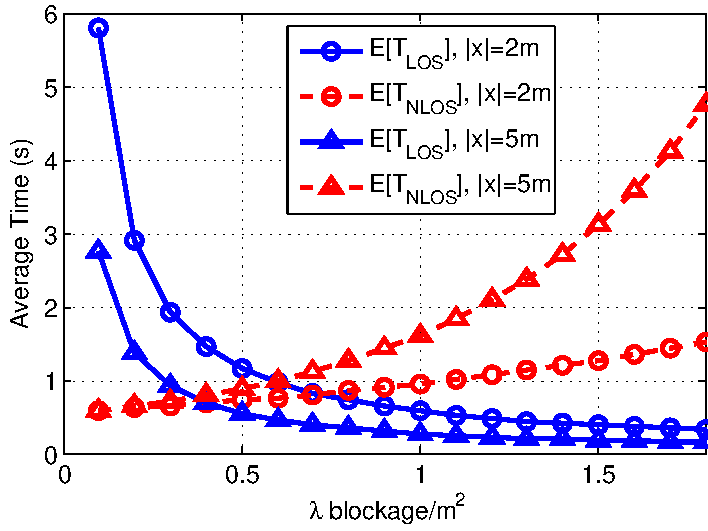
\includegraphics[width=0.4\textwidth]{Channel_constant_velocity_model.pdf} }
	
	\subfloat[State change frequency $f_{\mathrm{change}}$]{\label{subfig:freq} 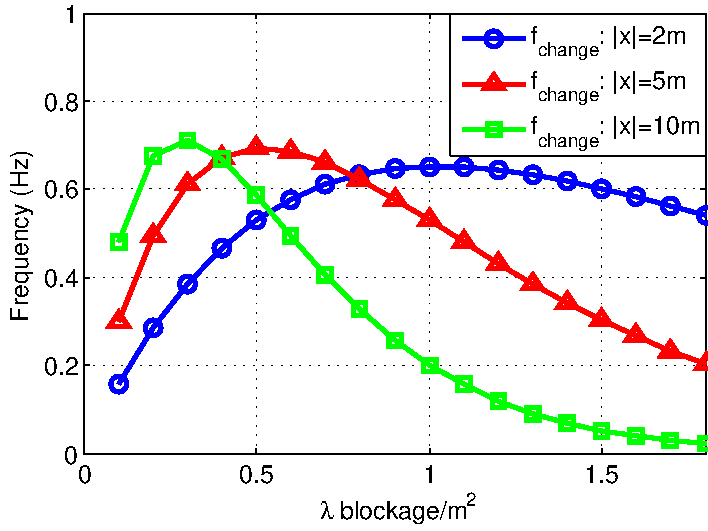
\includegraphics[width=0.4\textwidth]{Channel_constant_velocity_model_frequency.pdf}}
	
	\caption[]{$\E[T_{\LOS}]$, $\E[T_{\NLOS}]$ and $f_{\mathrm{change}}$ for different $\lambda$ and $|x|$. User's average velocity is $\E[s] = 1$m/s. Blockage is modeled as a rectangle of size $0.45\mathrm{m}\times 0.25\mathrm{m}$ and the width towards moving direction is $D_0=0.45\mathrm{m}$. }
	\label{fig:Channel_constant_velocity_model}
\end{figure}
In Fig. \ref{fig:Channel_constant_velocity_model} we present how $\E[T_{\LOS}]$, $\E[T_{\NLOS}]$ and $f_{\mathrm{change}}$ changes for different blockage density $\lambda$ and channel lengths $|x|$. From (\ref{eq:T_LOS}) we know that $\E[T_{\LOS}]$ is inversely proportional to $\lambda\E[s]|x|$ if we ignore $D_0$. Results in Fig. \ref{fig:Channel_constant_velocity_model}\subref{subfig:et} indicate that if the blockage density is higher, the blockages move faster and the link is longer, then the time of having LOS channel decreases while the time of having NLOS channel increases. Results in Fig. \ref{fig:Channel_constant_velocity_model}\subref{subfig:freq} indicate that the state of channel changes most frequently at moderately high user densities. 
By (\ref{eq:frequency}) we know that $f_{\mathrm{change}} \propto \E[S]$, thus different $\E[S]$ will not change the density that maximizes $f_{\mathrm{change}}$.
In dense wearable networks, distant users are likely to be blocked, i.e., $\mathrm{P_{LOS}}$ is small. Furthermore, the frequency that the channel becomes LOS $f_{\mathrm{change}}$ and the duration of $\LOS$ period is small, thus users may ignore distant fixed users when mitigating interference.

\appendix[Proof of generalised Steiner formula]
In this part we present the proof of generalized Steiner formula in \cite{stochasticapp}. We first introduce some related concepts.

Consider a $d$-dimensional space. 
$b(0,r)$ is a $d$-dimensional ball centered at origin with radius $r$.
$b_k$ is the volume of unit ball in dimension $k$, with $b_0$ = 1, $b_1$ = 2, $b_2$ = $\pi$, $b_3 = 4\pi/3$,  etc.

$V_k(K)$ is the intrinsic volume of set $K$ in dimension $k$, defined by mixed volumes.
The intrinsic volumes related to $d=2$ case include,
\begin{align*}
V_0(K) & = 1, \\
V_{d - 1}(K) & = \frac{1}{2}\nu_{d-1}(\partial K), \\
V_{d}(K) & = \nu_d(K),
\end{align*}
where $\nu_k$ is the measure in dimension $k$, $\partial K$ is the surface of $K$.

The proof requires the following two lemmas. 
\begin{lemma}\label{lemma:characterization}
	(Hadwiger's Characterization Theorem) Every non-negative, motion-invariant, monotone, C-additive convex body function $h$ can be written in the form, 
	\begin{equation}\label{characterization}
	h(K) = \sum\limits_{k=0}^{d}a_kV_k(K),
	\end{equation}
	where $a_k$'s are non-negative constants depending on $h$.
\end{lemma}
\begin{lemma}\label{lemma:steiner}
	If the intrinsic volumes of $\Xi$, $V_k(\Xi)$, have finite first moments,
	\begin{equation*}
	\overbar{V}_k(\Xi) = \E[V_k(\Xi)]<\infty,
	\end{equation*}
	for $k=0,1,\ldots, d$, then Steiner formula is satisfied for $\Xi$ almost surely. For $r\geq 0$, 
	\begin{equation}
	\E[\nu_d(\Xi \oplus b(0,r))] = \sum\limits_{k=0}^{d}b_{d-k}\overbar{V}_k(\Xi)r^{d-k}.
	\end{equation}
\end{lemma}

With Lemma \ref{lemma:characterization} and Lemma \ref{lemma:steiner}, we can prove the generalized Steiner formula in the following theorem.
\begin{theorem}
	For convex and isotropic $\Xi$, $\Xi$ has a distribution invariant w.r.t. rotations about the origin $0$, the generalized Steiner formula holds for every compact convex set $K$. 
	\begin{equation}
	\E\big[\nu_d(\Xi\oplus K)\big] = \frac{1}{b_d}\sum\limits_{k=0}^{d}\frac{b_k b_{d-k}}{{d \choose k}}\overbar{V}_k(\Xi) V_{d-k}(K).
	\end{equation}
\end{theorem}
\begin{proof}
	$\Xi$ is convex and isotropic, thus $h(K)$ satisfies Lemma \ref{lemma:characterization}. Let $h(K) = \E[\nu_d(\Xi \oplus K)]$ then by (\ref{characterization}) we have, 
	\begin{equation}\label{characterization:steiner}
	\E[\nu_d(\Xi\oplus K)] = \sum\limits_{k=0}^{d}a_kV_k(K),
	\end{equation}
	where $a_k$'s are constants related to $k$ and $\Xi$ and (\ref{characterization:steiner}) holds for all $K$. 
	
	Let $K=b(0, r)$, then 
	\begin{equation}\label{characterization:ball}
	\begin{aligned}
	\E[\nu_d(\Xi\oplus b(0,r))] &= \sum\limits_{k=0}^{d}a_kV_k(b(0,r))\\
	& = \sum\limits_{k=0}^{d} a_k{d \choose k}\frac{b_d}{b_{d-k}}r^k,
	\end{aligned}
	\end{equation}
	for all $r\geq 0$.
	
	By Lemma \ref{lemma:steiner}, 
	\begin{equation}\label{steiner:ball}
	\begin{aligned}
	\E[\nu_d(\Xi\oplus b(0,r))] &= \sum\limits_{k=0}^{d}b_{d-k}\overbar{V}_k(\Xi)r^{d-k}\\
	& = \sum\limits_{k=0}^{d}b_k\overbar{V}_{d-k}(\Xi)r^k,
	\end{aligned}
	\end{equation}
	for all $r\geq 0$.
	
	By (\ref{characterization:ball}) and (\ref{steiner:ball}) and the equality of polynomials, we have 
	\begin{equation*}
	a_k{d \choose k}\frac{b_d}{b_{d-k}} = b_k\overbar{V}_{d-k}(\Xi),
	\end{equation*}
	for $k = 0, 1,\ldots, d$. Additionally ${d\choose k} = {d\choose {d-k}}$, thus
	\begin{equation}\label{ak}
	a_k = \frac{1}{b_d}\frac{b_kb_{d-k}}{{d\choose {d-k}}}\overbar{V}_{d-k}(\Xi),
	\end{equation}
	for $k = 0, 1,\ldots, d$. Replace the $a_k$ in (\ref{characterization:steiner}) with (\ref{ak}) then we prove the theorem.
\end{proof}

\begin{thebibliography}{50}

\bibitem{humanactivity}
S. Collonge, G. Zaharia and G.E. Zein, ``Influence of human activity on wide-band characteristics of the 60 GHz indoor radio channel,'' \emph{IEEE Trans. Wirel. Commun.}, vol. 3,  no. 6, pp. 2369-2406, 2004.

\bibitem{timevaryingpathshadowing}
I. Kashiwagi, T. Taga and T. Imai, ``Time-varying path-shadowing model for indoor populated environments,'' \emph{IEEE Trans. Veh. Technol.}, vol. 59, no. 1, Jan. 2010.

\bibitem{blockagein60ghz}
S. Singh, F. Ziliotto, U. Madhow, E. M. Belding and M. Rodwell, ``Blockage and Directivity in 60 GHz Wireless Personal Area Networks: From Cross-Layer Model to Multihop MAC Design,'' \emph{IEEE J. Sel. Areas Commun.}, vol. 27, no. 8, Oct. 2009.

\bibitem{stochasticgeometry}
F. Baccelli and B. Blaszczyszyn, ``Stochastic geometry and wireless networks, volume \Rom{1} - theory,'' \emph{Foundations and Trends in Networking}, vol. 3, no. 3-4, pp. 249-449, 2009.

\bibitem{poisson}
J. F. C. Kingman, ``Poisson Processes,'' New York: The Clarendon Press Oxford Univ. Press, 1993.

\bibitem{stochasticapp}
S.N. Chiu, D. Stoyan, W.S. Kendall and J. Mecke, \emph{Stochastic Geometry and its Applications} (3rd ed). Hoboken: Wiley, 2013. 

\bibitem{busyperiod_heavytraffic}
P. Hall, ``Heavy Traffic Approximations for Busy Period in an M/G/$\infty$ Queue,'' \emph{Stochastic Processes and their Applications}, vol. 19, no. 2, pp. 259-269, 1985.

\bibitem{busyperiod_exponential}
M. A. M. Ferreira and M. Andrade, ``The M/G/$\infty$ Queue Busy Period Distribution Exponentiality,'' \emph{Applimat - Journal of Applied Mathematics}, vol. 4, no. 3, pp. 249-260, 2011.


\end{thebibliography}

\end{document}
